% ************ Chapter 2 ************
%\renewcommand{\chaptername}{Chapter}
\chapter{Estado da Arte \label{chapter_estado_arte}}
\label{cap:2}

O tema descentralização da \emph{Web} não é novo, existindo até ao momento alguns projetos relevantes nesta área.
Este capitulo consiste numa apresentação mais detalhada sobre a alternativas que demonstram mais potencial.
É expectável que os detalhes estudados e apresentados permitam tirar mais conclusões no capitulo correspondente à análise de valor.

Assistimos hoje em dia a problemas sérios e crescentes relativos a manipulação de informação, consequentes de um paradigma de \emph{Web} que foi explorado ao limite, por forma a criar modelos de negócio obscuros e com pouca transparência na recolha e utilização dos dados de utilizadores.

O modelo atual é um autêntico colosso, onde a informação se encontra replicada infinitamente, e a camada de persistência de dados nas diferentes arquiteturas é provavelmente aquela que mais destaque tem para todas as estruturas organizacionais, na medida em que persiste o ativo principal das empresas, os dados relativos a toda a atividade todos seus clientes\cite{top_three_issues_centralized_web}. Isto torna-se um problema, quando não existe respeito pelos utilizadores e a manipulação dos dados passa a ser o \emph{“core business”}. Esta manipulação pode ser positiva, no sentido de criar valor para a empresa e para o cliente, ou pode ser negativa se estiver perante casos de uso de que coloquem em risco a privacidade ou que cedam os dados a terceiros não devidamente autorizados \cite{facebook_data_hell_medium}.

Um modelo de descentralização da web, vem sendo discutido desde tempos atrás, com várias abordagens possíveis, mas sempre com a garantia de que a informação será, em qualquer circunstância, propriedade do utilizador\cite{why_web_decentralization_future}.
A emersão de um novo modelo para a \emph{Web} está dependente de uma migração massiva do “antigo” para o novo, na medida em que estaria pendente da aceitação de plataformas digitais com infraestruturas de dimensão considerável e de toda a comunidade de engenharia informática. Esta adoção massiva por sua vez requer um conjunto de ferramentas capazes de sustentar o seu funcionamento de forma eficaz e suficientemente escalável \cite{shift_power_to_users}.

\section{Modelos Descentralizados \label{section_modelos_descentralizados}}
Nesta secção são apresentadas diferentes alternativas que podem servir de base para um novo paradigma de \emph{Web} descentralizada. E, como tal, são soluções robustas que oferecem ferramentas auxiliares para o desenvolvimento e posterior integração de novas aplicações.

\subsection{Solid \label{estado_arte_solid}}
Um dos conceitos fundamentais do \emph{Solid} é o \emph{Personal online datastore \label{sym:POD}} (\emph{POD}), este, na sua definição, é a unidade de armazenamento de recursos no \emph{Solid}, recursos estes que pertencem a utilizadores e que poderão, com as devidas autorizações, ser utilizados por outras aplicações cliente.

A arquitetura implícita para o desenvolvimento de aplicações baseadas em Solid permite que os utilizadores escolham um \emph{POD} à sua escolha, podendo este ser próprio ou recorrendo a um servidor partilhado para conceder às aplicações autorização para armazenar ou ler informação a partir do mesmo. Por si só, este facto permite que os utilizadores escapem dos tradicionais “silos de dados”. Além disto, esses PODs podem oferecer diferentes granularidades de privacidade, confiabilidade, disponibilidade, proteção legal e reutilização de dados\cite{solid_official}. Desta forma, este componente do Solid confere a camada de persistência de informação dos utilizadores, podendo inclusive ser visto como o novo \emph{backend} das aplicações, que poderão aceder à informação através da interface \emph{REST}\cite{rest_foundations} disponibilizada por cada POD, baseada em Linked Data Platform (LDP \label{sym:LDP}), uma recomendação da comunidade W3C, assim como um mecanismo baseado em queries SPARQL\cite{solid_spec}.

\subsubsection{Autenticação \label{section_estado_arte_solid_authentication}}
A identidade dos utilizadores no Solid baseia-se em URIs WebID, estes funcionam como nomes universais que permitem identificar determinado utilizador de forma descentralizada. Segue-se um exemplo de um possível WebID:

\begin{center}
    \emph{https://john.domain.com/profile/card\#me}
\end{center}

Neste sentido, o Solid, tratando-se de uma plataforma descentralizada, tem requisitos diferentes da maioria das aplicações existentes. Precisa de estar assente em mecanismos de autenticação \emph{cross-domain} suficientemente descentralizados e isolados de qualquer serviço ou entidade\cite{solid_spec}.

Até ao momento, o mecanismo de autenticação a ser utilizado em determinada instância de um \emph{POD}, pode ser um de dois: \emph{WebID-TLS} ou \emph{WebID-OIDC}. Esta capacidade de abstração do mecanismo de autenticação, permite que possam continuamente ser estudados e adotados novos mecanismos que se entendam relevantes\cite{solid_spec}.
\newpara
\textbf{\emph{WebID-TLS}} foi o primeiro mecanismo de autenticação a ser implementado no Solid. Como forma de autenticar os \emph{WebIDs}, em vez das tradicionais \emph{passwords}, recorre a certificados criptográficos (guardados e geridos no navegador \emph{Web} do utilizador) para comprovar a identidade do utilizador\cite{solid_webid-tls:}.

Este mecanismo, apesar de poder ainda ser utilizado, deixou de ser a configuração por omissão para instanciações de novos PODs. Isto, porque muitos navegadores \emph{Web} removeram suporte ao elemento \emph{KEYGEN}, que servia como base para este protocolo gerar certificados através do navegador \emph{Web}\cite{solid_webid-tls:}.

\newpara
\textbf{\emph{WebID-OIDC}} é também um mecanismo de autenticação baseado \emph{WebID}, tendo a particularidade de ser baseado no protocolo \emph{OpenID connect} (\emph{OIDC}). 

Este mecanismo adiciona ao fluxo normal de \emph{OIDC} um passo extra que permite obter um URI \emph{WebID} através de um \emph{token} \emph{OIDC}\cite{solid_webid_oidc}.

Seguem-se alguns dos conceitos mais relevantes neste protocolo:
\begin{itemize}
    \item \emph{User} - Utilizador humano (pode ser também uma aplicação ou serviço se estes tiverem o seu próprio \emph{webID}). Também chamado \emph{Resource Owner};
    \item \emph{User-Agent} - Nome formal para navegador \emph{Web};
    \item \emph{Identity Provider (OP)} - Um servidor de identidade baseado no protocolo \emph{OpenID Connect}. Pode ser utilizado o próprio \emph{POD} uma instância externa;
    \item \emph{Resource Server} - Um servidor responsável por alojar recursos que o utilizador precisa eventualmente de aceder, tais como \emph{HTML}, imagens, \emph{Linked Data} / \emph{RDF sources}, entre outros tipos de recursos;
    \item \emph{Relying Party (RP)} - É um \emph{POD} ou uma aplicação cliente que assenta a sua lógica num \emph{token} providenciado por um servidor de identidade;
    \item \emph{POD} - Unidade online de armazenamento pessoal. Este componente do sistema desempenha vários papéis na arquitetura atual: armazena informação do utilizador (actua como \emph{Resource Server}), instancia um servidor de identidade \emph{webID-OIDC} e pode também actuar como \emph{Relying Party} quando um utilizador requisita recursos a partir de um \emph{token}.
\end{itemize}



Conforme é possível perceber pela figura \ref{web-id-oidc-sequence-diagram}, assemelha-se bastante ao protocolo OpenID Connect (figura \ref{open-id-connect-sequence-diagram}, adicionando dois passos extra\cite{solid_webid_oidc}:
\begin{itemize}
    \item Obter o \emph{WebID} através do \emph{token} de acesso;
    \item Verificar se o servidor indicado para autenticação é de facto o servidor de identidade autorizado para o \emph{WebID} em questão.
\end{itemize}


\begin{figure}[H]
    \centering
    % Requires \usepackage{graphicx}
    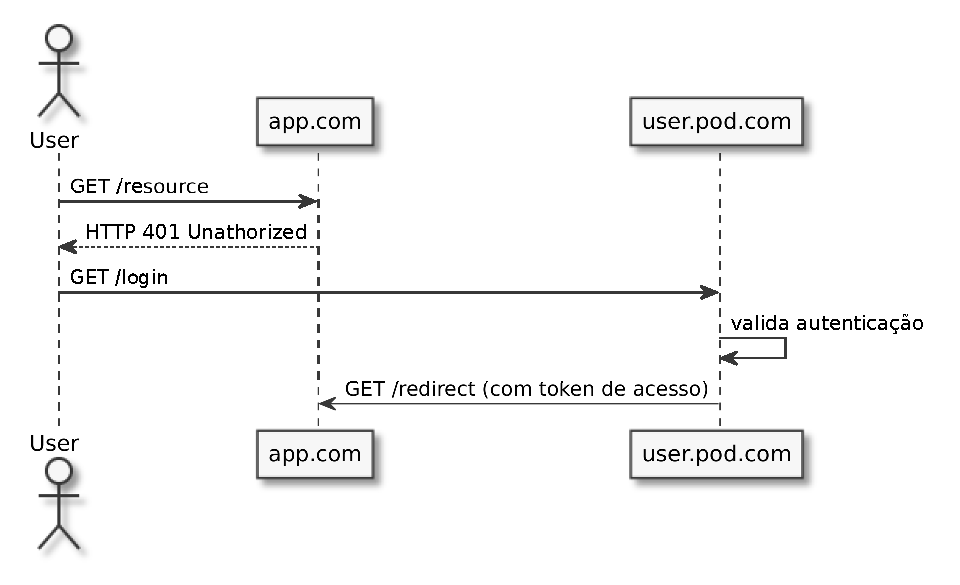
\includegraphics[width=0.9 \textwidth]{figures/open_id_connect_sd.eps}
    \caption{Diagrama de sequência \emph{OpenID Connect}}
    \label{open-id-connect-sequence-diagram}
\end{figure}

\begin{figure}[H]
    \centering
    % Requires \usepackage{graphicx}
    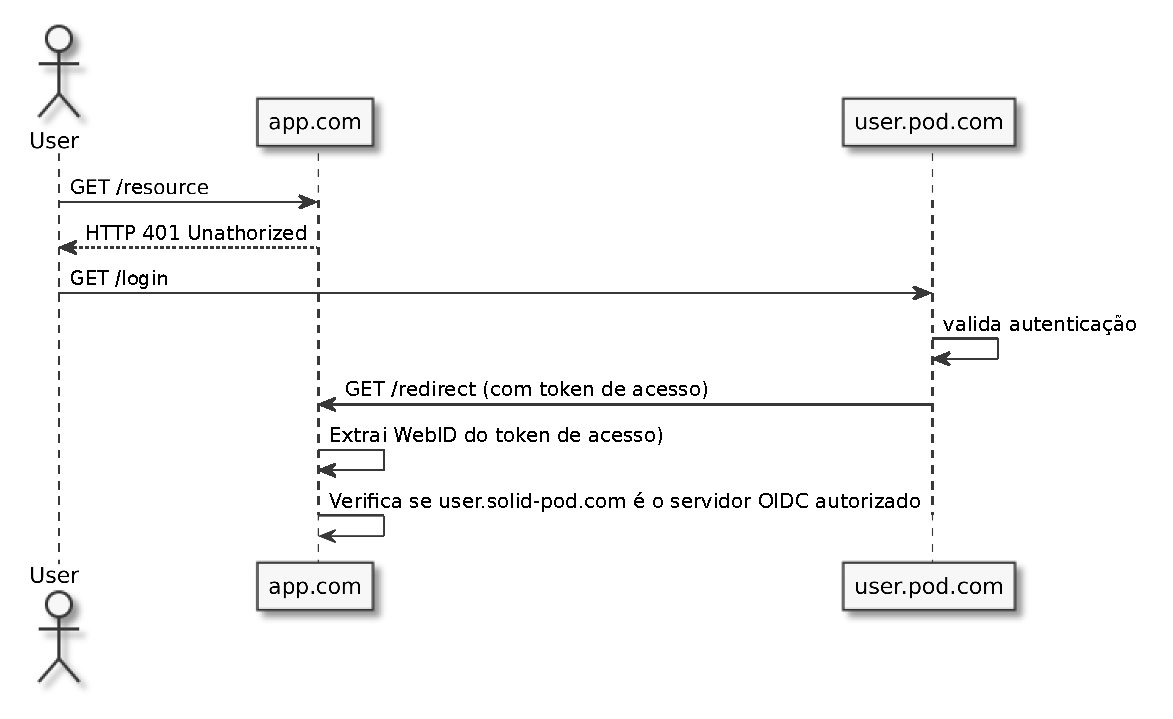
\includegraphics[width=0.9 \textwidth]{figures/WebId-OIDC}
    \caption{Diagrama de sequência \emph{WebID-OIDC}}
    \label{web-id-oidc-sequence-diagram}
\end{figure}

\subsubsection{Autorização}
A autorização no Solid é garantida por um componente com o nome \emph{Web Access Control (WAC)}. Este componente consiste num sistema de controlo de acesso entre domínios de origem cruzada. Os seus conceitos principais baseiam-se em modelos de controlo de acesso a diferentes sistemas de ficheiros e as suas principais responsabilidades consistem em garantir acesso a agentes (utilizadores, grupos, entre outros) para conseguirem realizar ações (ler, escrever, editar, eliminar, entre outras)\cite{solid_web_access_control}.
Seguem-se algumas das suas principais características:
\begin{itemize}
    \item Os recursos são identificados por URLs, e podem referir-se a qualquer recursos disponível na \emph{Web};
    \item As politicas de controlo de acesso seguem uma estrutura declarativa;
    \item Utilizadores e grupos são também identificados URLs (WebIDs);
    \item Agnóstico em termos de domínio, ou seja, as politicas de acesso a um determinado ficheiro podem conter utilizadores e grupos alojados em qualquer servidor de identidade existente.
\end{itemize}

\subsubsection{Armazenamento \label{subsection_solid_armazenamento}}
O \emph{POD} representa o componente que lida com toda a gestão de recursos do utilizador através da disponibilização de uma interface de aplicação \emph{REST} (\emph{c.f.} \ref{estado_arte_representacao_solid}). Este componente permite ao \emph{Solid} suportar dois tipos de informação:
\begin{itemize}
    \item Recursos \emph{Linked Data}, que podem recorrer às capacidades implícitas no Solid para aplicar lógica no lado da aplicação cliente;
    \item Todo o restante tipo de informação, como por exemplo imagens, documentos, vídeos, áudio, etc.
\end{itemize}

Desta forma, é possível construir aplicações baseadas em Solid com ou sem recursos sob a forma de \emph{Linked Data}\cite{solid_spec}.

Os recursos são agrupados em contentores baseados em directórios (cumprindo a especificação \emph{LDP Basic Container Spec}\cite{solid_spec}.

\begin{figure}[H]
    \begin{center}
    % Requires \usepackage{graphicx}
    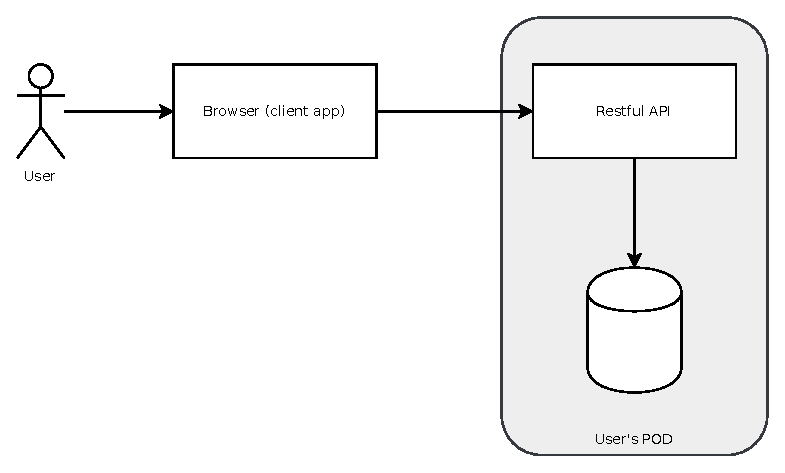
\includegraphics[width=0.8\textwidth]{figures/estado_arte-Solid.eps}
    \caption{Representação arquitetura \emph{Solid}}
    \label{estado_arte_representacao_solid}
    \end{center}
\end{figure}


\subsection{Blockstack}
Blockstack é um projeto \emph{open-source} que pretende construir uma rede de computação descentralizada assente na camada de transporte da Internet e protocolos de comunicação subjacentes. Para atingir este estatuto, está assente nas seguintes camadas:
\begin{itemize}
	\item Stacks Blockchain - Permite aos utilizadores controlar e registar ativos digitais, como \emph{usernames} e \emph{passwords} ou executar contratos inteligentes\cite{blockstack_white_paper};
	\item Gaia - Armazenamento descentralizado;
	\item \emph{Blockstack Authentication} - Protocolo que permite autenticação descentralizada.\cite{blockstack_white_paper};
	\item Bibliotecas e \emph{SDKs} - Ferramentas para facilitar o desenvolvimento de aplicações baseadas em Blockstack\cite{blockstack_white_paper}.
\end{itemize}

\subsubsection{Autenticação}
Em termos de autenticação, o Blockstack consegue providenciar autenticação descentralizada através do mecanismo de autenticação por chave pública criptográfica. 

A partir do login, a aplicação recebe três componentes essenciais de informação: o nome de utilizador, uma chave privada específica de aplicação e a localização do repositório para armazenar informação\cite{blockstack_white_paper}.

\subsubsection{Autorização}
Os pedidos \emph{REST} para aceder a informação de determinado utilizador devem ser acompanhado por um \emph{token} de autenticação assinado e validado pelo repositório. Cada aplicação tem uma chave privada que confere acesso a uma partição especifica do repositório impedindo que, ao contrário do Solid, possa haver partilha de informação entre as diferentes aplicações.

\subsubsection{Armazenamento}

Um dos conceitos chave da arquitetura desta plataforma é o sistema de ficheiros descentralizado chamado Gaia Hub, que permite aos utilizadores escolher e providenciar o seu repositório de informação, podendo estes ser partilhados entre a comunidade ou ser propriedade de cada utilizador.

Estes repositórios disponibilizam uma interface de aplicação \emph{RESTful}, permitindo que as aplicações cliente devidamente autorizadas giram a informação do utilizador (\emph{c.f.} figura \ref{estado_arte_representacao_blockstack}).

Sendo que cada pedido deve ser acompanhado por um \emph{token} autenticação assinado e validado pelo repositório. Cada aplicação tem uma chave privada que confere acesso a uma partição especifica do repositório impedindo a partilha de informação entre as diferentes aplicações\cite{blockstack_white_paper}.

\begin{figure}[H]
    \begin{center}
    % Requires \usepackage{graphicx}
    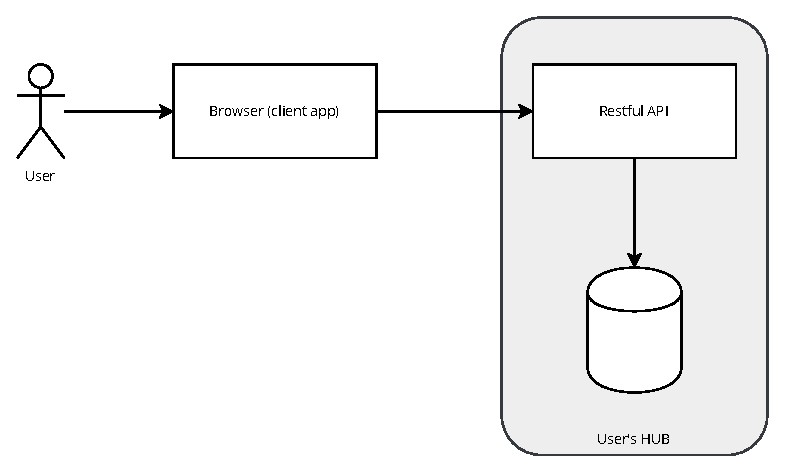
\includegraphics[width=0.8\textwidth]{figures/estado_arte-Blockstack.eps}
    \caption{Representação arquitetura Blockstack}
    \label{estado_arte_representacao_blockstack}
    \end{center}
\end{figure}

\subsection{Diaspora}
Diaspora é um projeto com uma visão um pouco mais reduzida que as restantes alternativas, na medida em que foca-se apenas em apresentar um protótipo daquilo que poderia ser uma rede social descentralizada. Este projeto assenta em servidores de informação independentes, que o utilizador pode escolher ou até mesmo configurar um por si próprio\cite{diaspora_wiki}.

\subsubsection{Autenticação}
Relativamente a autenticação, não é adotado nenhum mecanismo fora do comum, sendo apenas o método comum \emph{username/password}.

\subsubsection{Autorização}
No contexto de autorização, este projeto dispõe do conceito \emph{Aspect}, este permite criar regras de acesso a recursos para determinados conjuntos de utilizadores\cite{diaspora_wiki}.

\subsubsection{Armazenamento}
O conceito principal desta rede é o \emph{POD} (assim como no Solid), este representa o componente que gere e persiste a informação do utilizador. A informação entre todas as instâncias deste componente é mantida em sincronização utilizando a tecnologia \emph{WebSub}, conforme é possível observar na figura \ref{estado_arte_representacao_diaspora}\cite{diaspora_wiki}.

\begin{figure}[H]
    % Requires \usepackage{graphicx}
    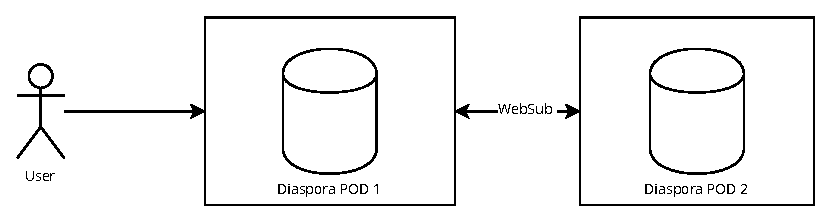
\includegraphics[width=0.8\textwidth]{figures/estado_arte-Diaspora.eps}
    \caption{Representação arquitetura Diaspora}
    \label{estado_arte_representacao_diaspora}
\end{figure}

\subsection{Elastos}
Elastos incide no desenvolvimento de um novo paradigma de \emph{Web} potenciado por tecnologia \emph{blockchain}\cite{a_bit_about_blockchain}. O foco principal incide não só na proteção dos dados, mas também na defesa dos direitos de autor. Conforme é possível ver na figura \ref{estado_arte_representacao_elastos}, a plataforma é constituída pelos seguintes quatro componentes:\cite{elastos_white_paper}
\begin{itemize}
	\item Elastos Blockchain;
	\item Elastos Runtime;
	\item Elastos Carrier;
	\item Elastos SDK.
\end{itemize}

O conceito baseia-se num sistema operativo relativamente leve que armazena a informação e previne que as aplicações e serviços tenham ligação direta Internet, sendo esta intermediada por meio do componente \emph{Elastos Carrier}. 

Toda a informação tem identificadores providenciados por Blockchain (pode ser Bitcoin ou uma rede de Blockchain alternativa \footnote{Qualquer outra rede Blockchain, não necessariamente a que serve de base à conhecida criptomoeda Bitcoin}), sendo estes IDs verificados antes de os ativos digitais serem transmitidos entre as diferentes máquinas virtuais, utilizando comunicação \emph{Peer to Peer} (\emph{P2P\label{sym:P2P}})\cite{what_are_P2P_networks} providenciada pelo \emph{Elastos Carrier}\cite{elastos_developer}.

\subsubsection{Autenticação}

Relativamente à autenticação, esta plataforma introduz um ID descentralizado (\emph{DID}\label{sym:DID}), construído na rede Blockchain, com a responsabilidade de providenciar identificadores seguros tanta para recursos como para utilizadores.

O identificador pode ser utilizado para efeitos de rastreamento, autenticação e estabelecimento de ligações seguras. De forma simplificada, o componente \emph{Elastos Carrier} é a combinação entre \emph{DID} e a comunicação \emph{P2P}, assegurando assim que a informação é transmitida em segurança após a autenticação e a autorização serem devidamente validadas\cite{elastos_white_paper}.

\subsubsection{Autorização}
A autorização neste projeto fica a cargo do componente \emph{Elastos Runtime}, este implementa em si um sistema que valida o acesso de determinado utilizador a determinado recurso\cite{elastos_white_paper}.

\subsubsection{Armazenamento}
Elastos dispõe de um componente de armazenamento descentralizado, i.e. Elastos Hive. Recorre a um sistema de arquivos interplanetário (\emph{IPFS}\label{sym:IPFS}) \cite{ipfs} como base. Oferece uma interface de aplicação para aceder à informação que será dispersa pelas diferentes regiões do planeta, garantindo assim fiabilidade às aplicações.\cite{elastos_white_paper}

\begin{figure}[H]
    % Requires \usepackage{graphicx}
    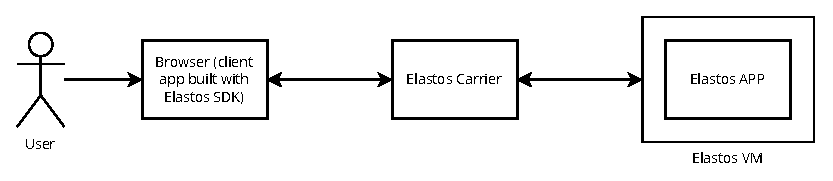
\includegraphics[width=0.8\textwidth]{figures/estado_arte-Elastos.eps}
    \caption{Representação arquitetura \emph{Elastos}}
    \label{estado_arte_representacao_elastos}
\end{figure}

\subsection{Comparação Modelos Descentralizados}

De forma a resumir, numa perspetiva de comparação, a informação apresentada sobre os diferentes modelos, estes são, de seguida, expostos na  na tabela \ref{tabela_comparacao_modelos_descentralizados}, tendo por base três tópicos:
\begin{itemize}
    \item Autenticação - De que forma os modelos descentralizados superam a necessidade validar a identidade do utilizador;
    \item Autorização - O mecanismo utilizado para garantir que o acesso restrito de um utilizador a determinado recurso;
    \item Armazenamento - Num contexto de descentralização, como é a garantido o acesso a determinado recurso.
\end{itemize}

\begin{center}
\small
\begin{longtable}{c|p{4cm}|p{4cm}|p{4cm}}
\caption{Tabela de comparação entre modelos descentralizados}
\label{tabela_comparacao_modelos_descentralizados}
\\
\toprule 
    \multicolumn{1}{c}{-} &
    \multicolumn{1}{c}{Autenticação} &
    \multicolumn{1}{c}{Autorização} &
    \multicolumn{1}{c}{Armazenamento}
    \\ \midrule\addlinespace[2pt] \endhead
\bottomrule\endfoot
\endlastfoot

Solid & Os utilizadores são identificados através de um WebID. Autenticação baseada em camada abstrata que permite utilizar o protocolo WebID-TLS ou WebID-OIDC \cite{solid_spec}. &  Garantida por um sistema WAC (\emph{Web Access Control} \label{sym:WAC}). Este sistema por sua vez é composto por documentos que contêm regras sobre a forma declarativas, denominadas ACLs \label{sym:ACL}, que indicam o tipo de acesso que cada WebID tem a determinado recurso \cite{solid_web_access_control}. & PODs disponibilizam uma camada de persistência baseada em LDP. Esta camada é acessível através de uma interface REST. \cite{solid_spec} \\
Blockstack & Autenticação descentralizada através do mecanismo de autenticação por chave pública criptográfica \cite{blockstack_white_paper}. & Chave privada específica de aplicação confere o acesso a determinada partição do repositório e, consequentemente, aos seus recursos \cite{blockstack_white_paper}. & Sistema de ficheiros descentralizado chamado Gaia Hub, que permite aos utilizadores escolher e providenciar o seu repositório de informação \cite{blockstack_white_paper}. \\
Diaspora & Não é adotado nenhum mecanismo fora do comum, sendo apenas o método comum username/password \cite{diaspora_wiki}. & Autorização de acesso baseada no conceito \emph{Aspect}, este funciona como um agrupador de utilizadores que tem acesso a um determinado recurso \cite{diaspora_wiki}. & Os diferentes PODs existentes pelo mundo conferem o funcionamento da rede social e mantêm-se sincronizados utilizando a tecnologia WebSub \cite{diaspora_wiki}. \\
Elastos & Introduz um ID descentralizado (DID), construído na rede Blockchain e providencia IDs confiáveis para tudo e para todos \cite{elastos_white_paper}. & A camada \emph{Elastos Runtime contém um sistema de gestão de permissões que confere ou o acesso de determinado utilizador a um recurso} \cite{elastos_white_paper} & Recorre a um sistema de arquivos interplanetário (IPFS) como base. \cite{elastos_developer}
\end{longtable}
\end{center}

\section{Métodos}
No decorrer do desenvolvimento do projeto, foram estudados e aplicados diferentes métodos, de forma a responder a diferentes necessidades surgidas. Neste contexto, os métodos consistem em todas as metodologias e técnicas utilizadas com vista a explorar conceitos. Estes tiveram principal impacto nas fase de análise, contribuindo para facilitar processos de decisão e estabelecer metas.

\subsection{New Concept Development}
O processo de inovação é divido em três componentes: \emph{Fuzzy
Front End}, o processo \emph{New Product Development} e comercialização \cite{fuzzy_frontend}. A Figura seguinte
apresenta o processo de inovação.

\begin{figure}[H]
    \begin{center}
    % Requires \usepackage{graphicx}
    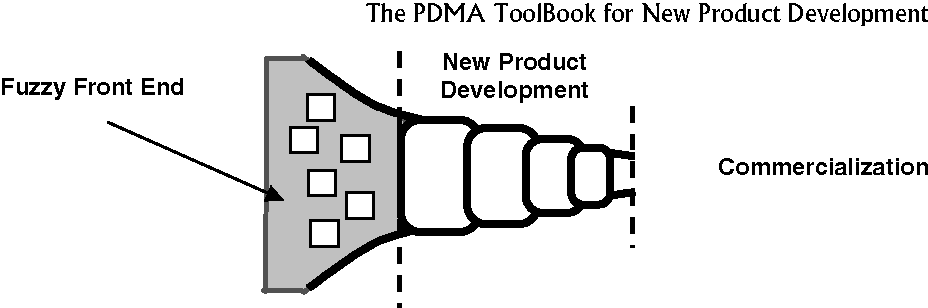
\includegraphics[width=1\textwidth]{figures/new_product_development.png}
    \caption{Representação Elastos}
    \end{center}
\end{figure}

O \emph{Fuzzy Front End} é a fase inicial do processo de desenvolvimento de novos produtos, correspondendo ao momento da identificação do problema ou à captação de oportunidades para o
projeto. Esta fase caracteriza-se por processos e decisões não estruturadas que tem como objetivo a identificação das necessidades dos potenciais clientes. A fase seguinte é o processo de  desenvolvimento do novo produto, sendo esta uma fase onde as ideias já estão mais estruturadas e os objetivos definidos. A terceira fase é a comercialização
do produto e corresponde à fase em que o produto é introduzido no mercado \cite{fuzzy_frontend}.

O modelo \emph{New Concept Development Model} é a representação das principais atividades do Fuzzy Front End. Este consiste em três componentes:

\begin{itemize}

\item Motor: Mecanismo que impulsiona as atividades de liderança e estratégia de negócio da organização;

\item Cinco Processos: São os processos que compõem o centro do modelo, que têm em conta a visão geral, a estratégia pretendida e a sua motivação;

\item Fatores de Influência: Variáveis não controláveis de origem interna ou externa ao projeto que afetam a sua inovação.

\end{itemize}

\begin{figure}[H]
    \begin{center}
    % Requires \usepackage{graphicx}
    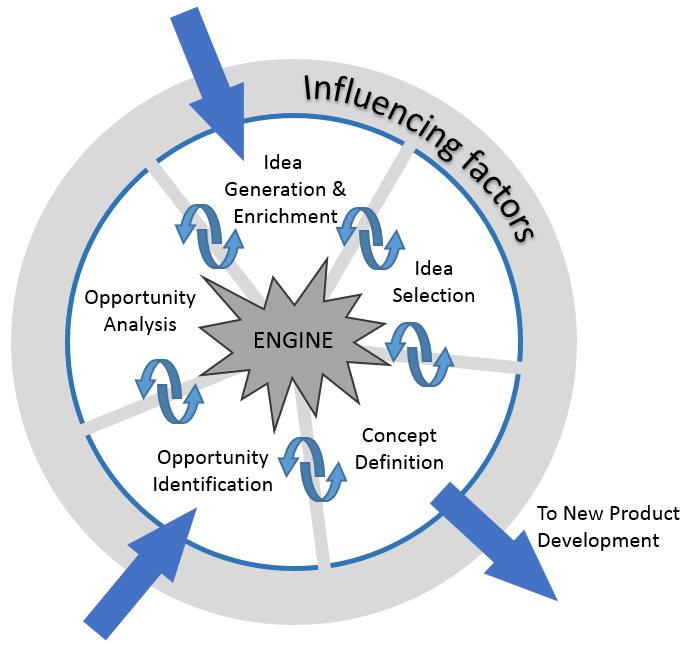
\includegraphics[width=0.5\textwidth]{figures/The-New-Concept-Development-NCD-model-Koen-et-al-2001.png}
    \caption{Representação New Concept Development Model}
    \end{center}
\end{figure}

O modelo apresenta duas vias de entrada e uma única saída, sendo este iniciado pela identificação de uma oportunidade ou pela geração de uma ideia. Essa irá posteriormente interagir com os restantes componentes do modelo.

\subsection{\emph{Analytic Hierarchy Process} (\emph{AHP})\label{section_AHP}\label{sym:AHP}}

Este método foi criado por Tomas L. Saaty em 1980, sendo um dos métodos mais conhecidos de apoio à decisão. O seu principio baseia-se em desconstruir a ideia em fragmentos cada vez mais pequenos de modo a tornar a sua análise mais fácil. Para atingir esse fim, o método divide-se em três fases: Divisão Hierárquica, Definição de Prioridades e Consistência \cite{ahp}.

A divisão hierárquica do AHP consiste na definição do objetivo, dos critérios de resolução do problema e, por último, nas alternativas que resolvem o problema. A lógica é que tendo este conceitos organizados hierarquicamente, conseguimos perceber a relação entre eles.

Depois da divisão hierárquica, é necessário definir prioridades entre os diferentes pares de critérios escolhidos. Esta priorização é subjetiva, sendo necessário calcular o índice de consistência de modo a validar a decisão. Para fazer a priorização de critérios é possível utilizar-se a tabela que apresenta a relação entre cada par de critérios utilizando a escala de Saaty. Esta escala consiste numa escala numerada de 1 a 9, em que 1 corresponde a uma igualdade de importância entre critérios, 3 corresponde a uma fraca diferença de importância e 9 corresponde a uma diferença de importância absoluta. 


Por fim, é necessário garantir a consistência da decisão, uma vez que a priorização dos critérios é baseada em opinião e é subjetiva. Para isso são calculados os
índice de consistência e a razão de consistência. Desta forma é possível medir a consistência. Se o resultado do cálculo do rácio de consistência for menor que 0.1, consideram-se os critérios consistentes.

\subsection{\emph{Function Analysis System Technique (FAST) \label{sym:FAST}}}

Este modelo permite apresentar de forma gráfica as relações entre as funcionalidades de um determinado projeto, produto, processo ou serviço, tendo por base as questões: “Como” e “Porquê?”\cite{fast}.

Esta técnica ajuda, desta forma, a pensar no problema de forma mais objetiva e orientar os objetivos do seu desenvolvimento em função das relações entre as funcionalidades \cite{fast}.


\subsection{Modelo de Negócio \emph{Canvas}}

O modelo de negócio Canvas foi apresentado por Alex Osterwalder na sua tese de doutoramento \emph{The Business Model Ontology - A Proposition In A Design Science Approach, em 2004}. Este modelo permite, através de uma representação gráfica, mostrar como determinada empresa vende o seu produto  e como ganha dinheiro \cite{canvas}.

\subsection{Avaliação \label{estado_arte_avaliacao}}
Avaliação consiste na medição ou avaliação de uma determinada grandeza, utilizando uma metodologia ou técnica específica de modo a validar ou refutar uma hipótese. Sendo, assim, para a realização de um teste de avaliação, a definição de grandezas, hipóteses e as metodologias de avaliação\cite{experimentation_principles}.

\section{Tecnologias}
As tecnologias, tendo por base os resultados dos processos de análise, servem como veículos para desenhar e atingir os resultados. Assim, são apresentadas, de seguida as tecnologias exploradas no seguimento deste projeto, as mesmas são separadas pelas seguintes categorias:
\begin{itemize}
    \item Arquiteturas
    \item Padrões
    \item Linguagens
    \item Ferramentas
\end{itemize}

\subsection{Arquiteturas}
Arquitetura de software corresponde ao processo de converter características de software como flexibilidade, escalabilidade, viabilidade, reutilização e segurança numa solução estruturada que permita responder às necessidades técnicas de negócio\cite{software_architecture}.

Apresentam-se, de seguida, nesta secção algumas das arquiteturas de software estudadas no âmbito desta dissertação.

\subsubsection{Arquitetura orientada a micro-serviços}

Uma arquitetura orientada a micros-serviços define uma configuração, na qual os componentes são aplicações independentes. Essas aplicações independentes comunicam utilizando \emph{RESTful Web Services} ou troca de mensagens \cite{building_microservices:2015}.
Seguem-se algumas características de sistemas orientados a micro-serviços\cite{monolith_to_microservices}:
\begin{itemize}
\item Micro-serviços em execução de forma independente;
\item Sistema é partido em micro-serviços, tendo por base \emph{bounded context} (\emph{c.f.} secção \ref{subsubsection:bounded:context} e/ou capacidades de negócio;
\item O conceito “produto” ganha relevo face ao conceito “projeto”;
\item Aplicações devem utilizar canais de comunicação relativamente simples, como protocolo \emph{REST} ou troca de mensagens;
\item Diferentes micro-serviços podem seguir arquiteturas e implementações diferentes, dependendo das suas especificidades e das decisões levadas a cabo pelas equipas de desenvolvimento;
\item Seguindo as boas práticas de desenvolvimento de micro-serviços, cada aplicação deve ter a sua própria unidade de persistência de dados, podendo inclusive a tecnologia adjacente à mesma ser diferente para cada micro-serviço;
\item \emph{Pipelines} de desenvolvimento independentes;
\item \emph{Deploys} independentes.
\end{itemize}

\subsubsection{Arquitetura cliente servidor \label{estado_arte_cliente_servidor}}
A arquitetura cliente servidor é aquela que é mais utilizada no desenvolvimento de Software à data desta dissertação. Nesta, existem tipicamente três camadas (\emph{c.f.} figura 4.1):

\begin{itemize}
    \item Cliente - Responsável por gerir interação com o utilizador final;
    \item Servidor - Camada detentora da lógica de negócio responsável por servir um ou mais clientes;
    \item Persistência - Responsável pela persistência dos dados
\end{itemize}

\begin{figure}[H]
    \begin{center}
    % Requires \usepackage{graphicx}
    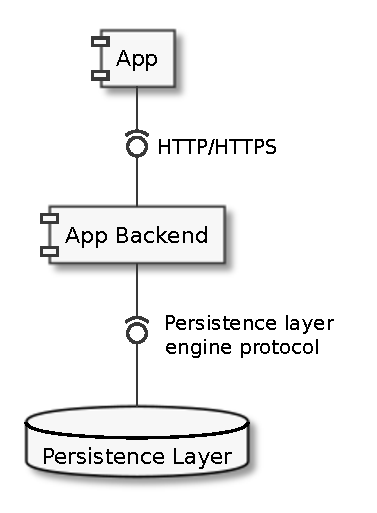
\includegraphics[width=0.5 \textwidth]{figures/actual_web.eps}
    \caption{Diagrama de Componentes Arquitetura Cliente Servidor}
    \end{center}
\end{figure}

\subsubsection{P2P \label{subsection:p2p}}
P2P é um formato de rede de computadores, cuja principal característica é descentralização das funções convencionais de rede. Neste conceito, o computador de cada utilizador conectado acaba por realizar simultaneamente as funções de servidor e de cliente\cite{what_are_P2P_networks}.

O seu principal objetivo é a transmissão de recursos e o seu surgimento possibilitou a partilha em massa de músicas e filmes \cite{what_are_P2P_networks}.

\subsection{Padrões}
Um padrão consiste numa solução que resolve sucessivamente um problema comum no contexto das diferentes fases de desenvolvimento de software, sendo nesta secção expostos padrões de desenho e padrões arquiteturais. Por norma um padrão não corresponde a uma solução final, mas sim a um guia ou um \emph{template} que pode ser adaptado a diferentes situações\cite{clean_architecture}.

\subsubsection{JWT \label{subsection:jwt}}
\emph{JSON Web Token} (\emph{JWT\label{sym:jwt}}) é um padrão (RFC-7519) da Internet. Este padrão define como devem ser transmitidos e armazenados objetos em formato JSON de forma compacta e segura entre diferentes aplicações. Um dos seus grandes fatores de adoção é o facto de ser assinado digitalmente, garantindo que os dados nele contidos podem ser validados a qualquer momento\cite{jwt_medium}.

O objeto deve ser constituído por três secções:
\begin{itemize}
    \item \emph{Header} - Esta secção indica o tipo de token e o o algoritmo de criptografia utilizado para a sua assinatura digital;
    \item \emph{Payload} - Contém todo objeto JSON inicialmente criado, este na maioria dos casos deverá conter informação sobre o utilizador autenticado;
    \item \emph{Signature} - Este campo tem como principal objetivo garantir a integridade do \emph{token}.
\end{itemize}

\subsubsection{\emph{Bounded Context}} \label{subsubsection:bounded:context}
\emph{Bounded Context} é um padrão crucial em \emph{Domain Driven Design}(\emph{DDD}\label{sym:DDD}). É o foco da fase de desenho de grandes modelos. Para lidar com grandes modelos, \emph{DDD} recorre a divisão em diferentes \emph{bounded contexts}. Estes tem como objetivo delimitar o domínio complexo em contextos baseados na intenção do negócio \cite{bounded_context}.

\subsubsection{\emph{REST}}
\emph{Representational State Transfer} (\emph{REST}\label{sym:REST}), é um estilo arquitetural que torna mais fácil a comunicação entre sistemas. Sistemas compatíveis com \emph{REST}, são caracterizados por manterem um elevado desacoplamento entre o cliente e o servidor.
Neste estilo arquitetural, as aplicações cliente fazem pedidos para obter ou alterar recursos em aplicações servidor, estes pedidos são constituídos por \cite{rest}:
\begin{itemize}
    \item Verbo HTTP - Define o tipo de ação a realizar, pode ser \emph{GET}, \emph{POST}, \emph{PUT}, \emph{PATCH} ou \emph{DELETE}
    \item \emph{Header} - Permite ao cliente passar detalhes sobre o pedido
    \item Caminho - URL onde o pedido deve ser respondido
    \item \emph{Body} - Mensagem que contém a informação sobre o recurso a ser criado ou alterado
\end{itemize}

\subsubsection{\emph{API Gateway}} \label{api_gateway}
Uma \emph{API Gateway} é uma interface que se situa entre a aplicação cliente e os micro-serviços. Esta interface é utilizada para criar uma camada de abstração entre as aplicações e as APIs providenciadas pelos diferentes micro-serviços, permitindo, assim, um elevado desacoplamento entre as diferentes APIs do sistema.

A adoção deste padrão confere ao sistema vantagens como as seguintes destacadas:
\begin{itemize}
    \item Escalabilidade - No futuro, a separação dos serviços existentes ou a criação de novos, não adicionará complexidade para além de alterar as regras de encaminhamento na API Gateway. Este componente pode inclusive contribuir para migrações controladas de tráfego entre serviços legados e novos;
    
    \item Segurança - A camada da API Gateway deverá centralizar responsabilidades como \emph{throttling} e inibição de tráfego com base em características do pedido (por exemplo IP de origem). O componente Solid-ID, não deverá estar “escondido” atrás da API Gateway, porque se trata de uma camada que deverá estar visível para o cliente, devendo esta ser utilizada para obter posteriormente acesso às funcionalidades expostas através da API Gateway.
\end{itemize}

\subsubsection{\emph{Troca de Mensagens Assíncrona}} \label{troca_mensagens_assincrona}
A troca de mensagens assíncrona consiste numa forma de troca de mensagens em que a aplicação que emite a mensagem não conhece o(s)seu(s) recetor(es), contribui para o incremento do desacoplamento entre as diferentes aplicações de um sistema.
Dois padrões associados a este mecanismo de troca de mensagens são \emph{Message Queueing} \emph{Publish/Subscribe}.

\emph{Message Queueing} \label{message_queueing} consiste num padrão em que as aplicações emissoras podem enviar para uma mesma fila, no entanto, existindo  apenas uma fila, qualquer mensagem poderá ser consumida apenas por um consumidor.

\begin{figure}[H]
    \begin{center}
    % Requires \usepackage{graphicx}
    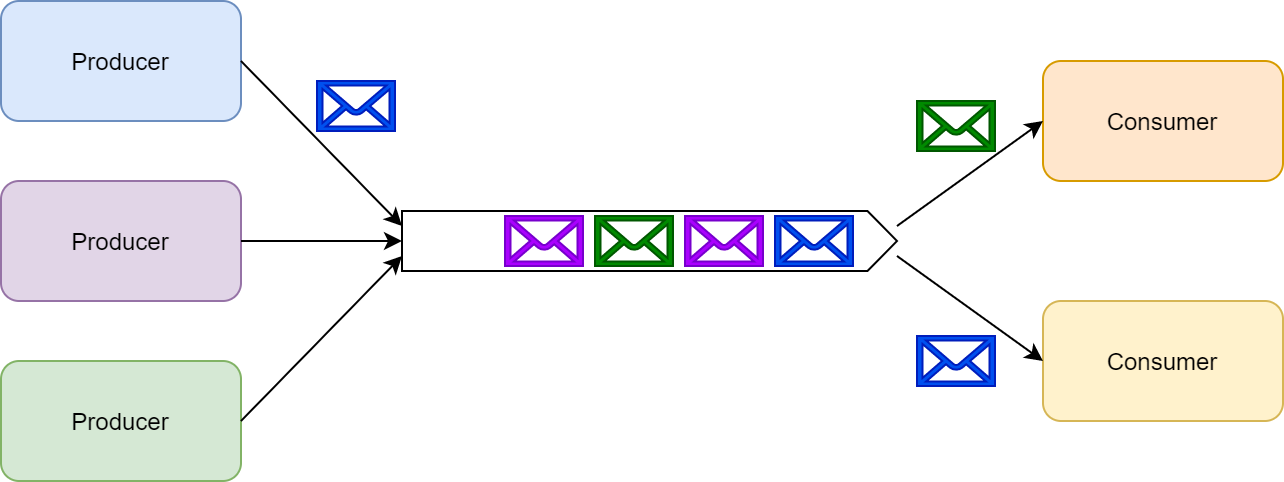
\includegraphics[width=1\textwidth]{figures/message_queueing.png}
    \caption{\emph{Message Queueing}}
    \end{center}
\end{figure}

\emph{Publish/Subscribe} \label{publish_subscribe} tem um comportamento idêntico ao padrão \emph{Message Queueing}, adicionando a este uma camada que permite que a mesma mensagem seja enviada para mais do que uma fila.

\begin{figure}[H]
    \begin{center}
    % Requires \usepackage{graphicx}
    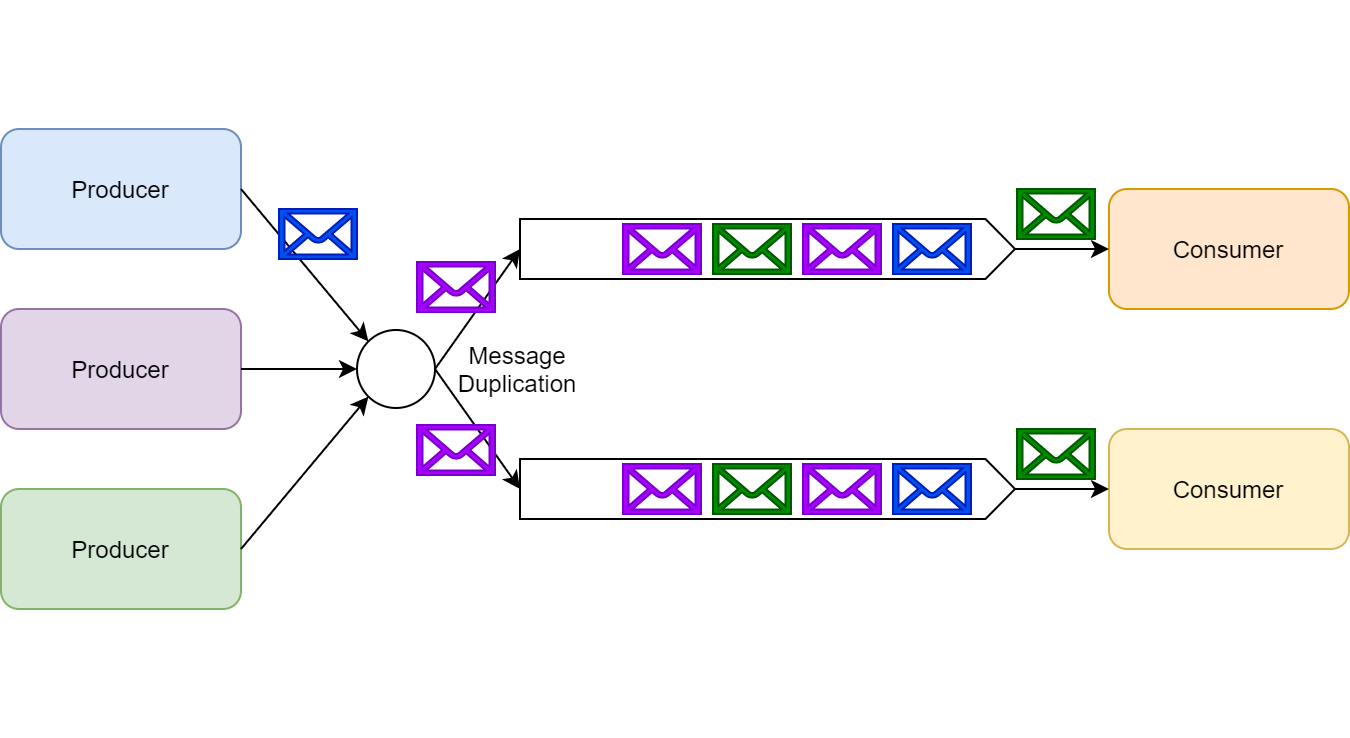
\includegraphics[width=1\textwidth]{figures/pub_sub.png}
    \caption{Publish/Subscribe}
    \end{center}
\end{figure}

\subsubsection{\emph{Command Query Responsability Segregation} (CQRS)} \label{cqrs}
Nas arquiteturas mais tradicionais, é utilizado o mesmo modelo de dados tanto para consultar como para atualizar a camada de persistência da aplicação. Esta abordagem é simples e funciona bem para operações CRUD básicas. Por outro lado, em aplicações mais complexas onde as cargas de leitura e de escrita são assimétricas, esta abordagem torna-se mais problemática e pode colocar em risco a escalabilidade do sistema. Neste contexto, o padrão CQRS incide em separar o modelo de leitura do modelo de escrita, existindo múltiplas abordagens para a sua implementação. \cite{cqrs}

\subsubsection{\emph{Service} \label{service_pattern}}
Este padrão indica que deve ser estabelecida uma camada na aplicação responsável por gerir a lógica de pedidos a serviços externos. Este padrão tem como principal objectivo abstrair a lógica de funcionamento dos diferentes serviço da lógica de negócio\cite{service_design_patterns}.

\subsubsection{Teorema \emph{CAP}} \label{cap_theorem}
O teorema \emph{CAP (Consistency, Availability, Partition) \label{sym:cap}} é uma ferramenta utilizada para ajudar a tomar decisões durante o desenho de sistemas distribuídos. Eric Brewer inferiu que em qualquer sistema distribuído existe um equilíbrio entre consistência, disponibilidade e tolerância a falhas. Afirmação corroborada em 2002 por Seth Gilbert e Nancy Lynch. O teorema afirma que sistemas distribuídos apenas podem garantir três das seguintes propriedades \cite{cap_theorem}:

\begin{itemize}
    \item Consistência - Garantia que qualquer nó num sistema distribuído retorna a mesma, mais recente, escrita com sucesso. Consistência consiste em qualquer cliente ter a mesma vista de determinada informação num determinado momento;
    \item Disponibilidade - Todos os nós funcionais retornam resposta para os pedidos de leitura e escrita num tempo razoável de resposta;
    \item Tolerância a falhas - O sistema continua a funcionar e mantêm consistência mesmo em cenários de falha de rede.
\end{itemize}

\subsubsection{\emph{Event Sourcing} \label{event_sourcing}}
\emph{Event sourcing} é um padrão que tem como objetivo garantir que as mudanças realizadas numa aplicação são armazenadas como uma sequência de eventos. Estes eventos persistidos, podem ser obtidos e utilizados para reconstruir estados da aplicação.
Neste sentido, este padrão é muitas vezes utilizado em conjunto com o padrão CQRS \cite{event_sourcing}.

\subsection{Linguagens}
Nesta secção incluem-se as linguagens de programação e modelação estudadas e utilizadas no decorrer da dissertação. Nesta secção incluem-se, portanto, linguagens que tiveram principal impacto no desenho e implementação da solução final.

\subsubsection{\emph{JavaScript} \label{estado_arte_javascript}}

\emph{JavaScript} é uma linguagem de programação criada em 1994 com o principal objetivo de adicionar funcionalidade e interação a \emph{web sites}. Assim, o \emph{JavaScript} foi originalmente desenhado para ser usado exclusivamente no \emph{front-end}, porém a introdução do \emph{engine V8} pela Google e, consequentemente, as melhorias de velocidade funcionalidade, introduziram não só o desenvolvimento de novas frameworks de \emph{front-end}, mas também uma nova linguagem de programação paradigma para o \emph{back-end}, o \emph{Node.js} (\emph{c.f. \ref{estado_arte_node_js}})\cite{javascript}.

\subsubsection{Node.js \label{estado_arte_node_js}}
Node.js pode ser considerado, mais do que uma linguagem de programação, um ambiente de execução multi-plataforma para JavaScript\cite{node_js}.

Uma das grandes particularidades do \emph{Node.js} é facto de não criar uma nova \emph{thread} para cada pedido, optando por adotar mecanismos assíncronos para lidar com operações de \emph{I/O}e, desta forma, prevenir que exista código bloqueante. Estes mecanismos conseguem garantir alto desempenho sem a necessidade de lidar com problemas de concorrência entre \emph{threads}\cite{node_js}.

\subsubsection{YAML}
\emph{YAML Ain't Markup Language} (\emph{YAML\label{sym:YAML}}) foi desenhada para ser uma linguagem com características capazes de a tornar fácil de perceção. Esta linguagem é maioritariamente utilizada em ficheiros de configuração em diversas ferramentas (e.g. docker) e frameworks (e.g. springboot)\cite{yaml}.

\subsubsection{UML}

\emph{Unified Modeling Language} (\emph{UML}\label{sym:UML}) é uma forma de criar representações visuais de um software, permitindo, também, fazer uma análise orientada a objetos através de notações gráficas. Foi inventada com objetivo de criar uma linguagem de modelação gráfica padrão para o design, arquitetura e execução de sistemas de software complexos\cite{uml}.

\subsection{Ferramentas}
Por ferramentas entende-se todas as aplicações e conjuntos de funcionalidades disponíveis com vista a criar valor nos diferentes processos de desenvolvimento\cite{software_tools}.

\subsubsection{\emph{RabbitMQ}}
\emph{RabbitMQ} é uma implementação de um \emph{Message Broker}, este suporta, de forma nativa, os dois padrão de de troca de mensagens assíncrona (\emph{c.f.} secção \ref{message_queueing} e \ref{publish_subscribe}). Para a implementação da lógica no sentido do padrão \emph{Publish/subcribe}, \emph{RabbitMQ} introduz o conceito de \emph{Exchange}, este componente é responsável por reencaminhar a mesma mensagem para as diferentes filas que subscreveram aquele tipo de mensagem.

\subsubsection{Apache Kafka}
\emph{Apache Kafka} por outro lado, é uma plataforma distribuída de streaming. Ao contrário de \emph{RabbitMQ}, que é baseado em filas e \emph{exchanges}, a camada de armazenamento do \emph{Kafka} é implementada utilizando transações de \emph{logs} particionadas.

Esta plataforma introduz o conceito de tópico. Um tópico representa uma categoria para a qual será mantida uma partição ordenada e imutável, de \emph{logs} com as mensagens recebidas.

\subsubsection{\emph{JMeter} \label{estado_arte_jmeter}}
\emph{JMeter} é uma ferramenta \emph{open-source} desenhada para realizar testes funcionais de carga, com vista a obter dados relativos a performance de determinado serviço\cite{jmeter}.

Esta ferramenta disponibiliza a funcionalidade de executar contra interfaces de aplicação REST através da configuração dos seguintes parâmetros\cite{jmeter}:
\begin{itemize}
    \item Caminho - O caminho que permite chegar ao serviço;
    \item Método - Método HTTP do \emph{endpoint} específico;
    \item Numero de \emph{Threads} - Cada \emph{thread} permite simular um utilizador a executar pedidos, sendo que múltiplas \emph{threads} irão ser executadas em paralelo e, por consequência, simular múltiplos utilizadores a fazer pedidos em simultâneo;
    \item Período \emph{Ramp-up}: Variável em segundos que indica quão gradual devem ser criadas novas \emph{threads}. A divisão do numero de \emph{threads} pelo valor configurado nesta variável indica o numero de novas \emph{threads} que serão criadas por segundo até que seja atingido o numero total;
    \item Total repetições - Numero de pedidos que cada \emph{thread} irá fazer. Assim que todas terminarem de executar o valor total de repetições, está concluído.
\end{itemize}

\subsubsection{\emph{Node Package Manager (NPM) \label{sym:npm}}\label{estado_arte_npm}}
\emph{NPM}, conforme sugere o nome, é um gestor de dependências \emph{Javascript}, que vem pré-instalado com o \emph{NodeJS}.
Esta ferramenta permite ligar-se a um repositório pré-definido ou configurar repositórios customizados, nestes é possível encontrar diferentes bibliotecas desenvolvidas e publicadas que podem ser utilizadas em novos projetos\cite{npm_explanation}.

\subsubsection{\emph{Containers} \label{estado_arte_containers}}
A tecnologia subjacente à utilização de \emph{Containers} consiste num mecanismo de criar uma espécie de contentor com o código base da aplicação e as suas dependências, e, posteriormente, este executar de formar isolada de outros processos.
Estes \emph{containers} podem partilhar o \emph{kernel} do sistema operativo, apresentando, assim, uma solução mais leve e robusta que as tradicionais máquinas virtuais \cite{techradar_containers}.






